\documentclass[12pt,fleqn]{article}

\usepackage[utf8]{inputenc}
\usepackage[T2A]{fontenc}
\usepackage[english,russian]{babel}
\usepackage{graphicx}
\usepackage{indentfirst}
\usepackage{syntax}
\usepackage{amsmath}
\usepackage{titlesec}
\usepackage{placeins}

\newcommand{\sectionbreak}{\clearpage}
\setcounter{secnumdepth}{0}

\begin{document}

\begin{titlepage}

\begin{center}
{\large
Санкт-Петербургский национальный исследовательский университет информационных технологий, механики и оптики

Факультет информационных технологий и программирования

Кафедра «Компьютерные технологии»\\[3cm]

И.А.Иванов\\[2cm]}

{\large \bfseries
Отчет по курсовой работе\\[0.5cm]

«Генерация LTL-формул по конечному автомату с помощью генетического программирования»
}
\vfill

Санкт-Петербург

2015
\end{center}

\end{titlepage}

\tableofcontents

\section{Введение}

Темпоральная логика (\emph{temporal logic}) \cite{tl} --- это логика, учитывающая причинно-следственные связи в условиях времени.
Используется для описания последовательностей явлений и их взаимосвязи по временной шкале.
Темпоральные логики часто применяются для выражения требований формальной верификации.
Например, свойства ``Если поступил запрос, то на него обязательно придет ответ''\ или
``Функция вызывается не более одного раза за вычисление''\ удобно формулировать с помощью темпоральных логик.
В линейной темпоральной логике (\emph{Linear Temporal Logic, LTL}) наряду с логическими операторами мы можем 
использовать следующие модальные операторы: утверждение истинно в следующем состоянии,
утверждение истинно всегда, утверждение когда-нибудь станет истинным,
одно утверждение будет истинным до тех пор, пока другое утверждение не станет истинным,
одно утверждение не станет ложным до тех пор (включительно), пока другое не станет истинным.

Задача нахождения спецификации (\emph{specification mining}) --- задача построения формальной спецификации или модели
(обычно автоматной) для некоторой программы. Существующие методы нахождения спецификации не позволяют получать темпоральные
формулы общего вида \cite{sm1, sm2, sm3, sm4}. В данной работе рассматривается способ построения спецификации
для управляющего конечного автомата в виде формул линейной темпоральной логики.
Управляющий конечный автомат характеризуется множеством состояний, входных событий, выходных воздействий,
а так же функцией переходов, каждый из которых описывается начальным состоянием, конечным состоянием,
входным событием, булевой формулой от входных переменных и множеством выходных воздействий.
Базовыми утверждениями, которые мы будем использовать являются следующие: произошло входное событие
\emph{e}, произошло выходное воздействие \emph{z}. Таким образом, мы будем искать формулы, удовлетворяющие автомату,
обладающие также некоторыми дополнительными свойствами. Во-первых, мы хотим, чтобы сгенерированные
формулы давали нам как можно больше информации о входном автомате.
Во-вторых, генерируемые формулы, в том числе предназначены для использования людьми, а значит не должны быть слишком громоздкими.
Позже эти требования будут формализованы.

В работе предлагается решение поставленной задачи с помощью генетического программирования --- класса алгоритмов,
которые решают задачи оптимизации путем подбора параметров с использованием механизмов, аналогичных естественному
отбору в природе, --- мутации, отбора и скрещивания.

\section{1. Постановка задачи}

\subsection{Управляющие конечные автоматы}

В работе управляющим конечным автоматом будем называть семерку $\langle X,\; E,\; Y,\; Z,\; y_0,\; \phi,\; \delta \rangle$,
где $X$ --- множество входных булевых переменных; $E$ --- множество событий; $Y$ --- множество состояний;
$y_0 \in Y$ --- начальное состояние; $Z$ --- множество выходных воздействий;
$\phi : Y \times E \times 2^X \rightarrow Y$ --- функция переходов, а
$\delta : Y \times E \times 2^X \rightarrow Z^*$ --- функция выходов.

\begin{figure}[!hb]
  \centering
    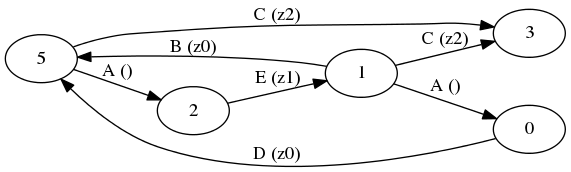
\includegraphics[scale=0.5]{lift.png}
  \caption{Пример управляющего автомата}
\end{figure}

\subsection{Формулы линейной темпоральной логики}

Язык LTL состоит из пропозициональных переменных, логических операторов $\wedge,\; \vee,\; \lnot,\; \rightarrow$\ и набора
темпоральных операторов, таких как, например, $G$\ (глобально в будущем), $X$\ (в следующий момент времени) и
$F$\ (когда-либо в будущем). Ниже приведена формула, утверждающая, что всегда в будущем из того, что верно $B$, следует,
что когда-либо в будущем будет верно $A$, и в следующий момент времени верно $C$:

$$
G(B \rightarrow F(A)) \wedge X(C).
$$

\subsection{Генетическое программирование}

В генетическом программировании особи, чаще всего, представляют в виде деревьев.
Оператор скрещивания реализуется обменом между двумя деревьями какими-либо узлами вместе с их
потомками. Оператор мутации может быть реализован изменением информации в узле, добавлением или удалением узла
или целого поддерева. Пусть, например, особи являются деревьями разбора формул пропозициональной логики.
Тогда оператор скрещивания для формул

\setcounter{topnumber}{10}
\setcounter{bottomnumber}{10}
\setcounter{totalnumber}{10}

\FloatBarrier

\begin{figure}[!h]
  \centering
    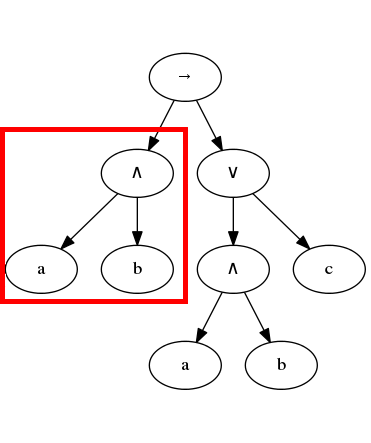
\includegraphics[scale=0.45]{t1.png}
\end{figure}

\begin{figure}[!h]
  \centering
    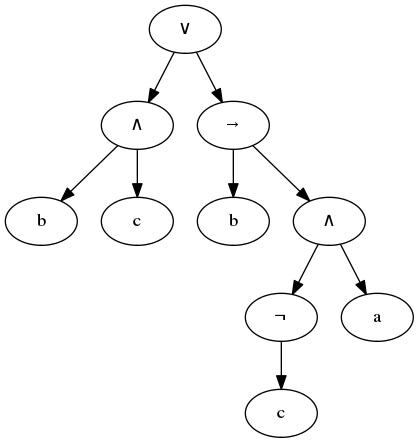
\includegraphics[scale=0.45]{t2.png}
\end{figure}

\FloatBarrier

мог бы выдать следующие результаты:

\FloatBarrier

\begin{figure}[!h]
  \centering
    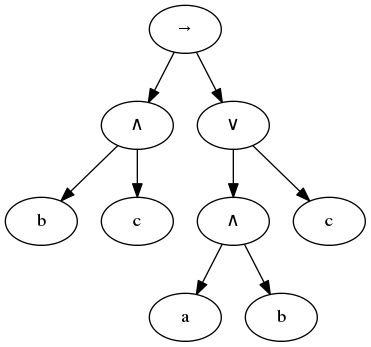
\includegraphics[scale=0.45]{t3.png}
\end{figure}

\begin{figure}[!h]
  \centering
    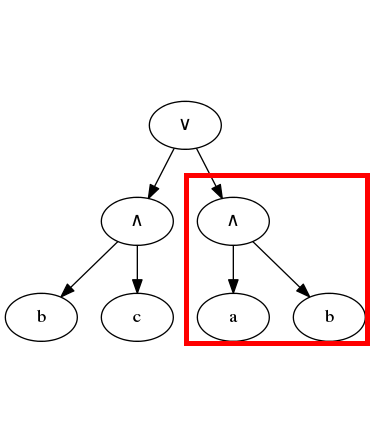
\includegraphics[scale=0.45]{t4.png}
\end{figure}

\begin{figure}[!h]
  \centering
    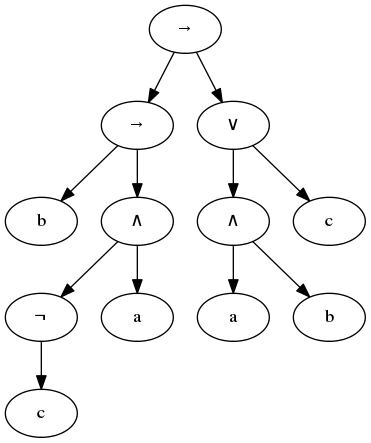
\includegraphics[scale=0.45]{t5.png}
\end{figure}

\FloatBarrier

А результатом применения оператора мутации к формуле

\FloatBarrier

\begin{figure}[!h]
  \centering
    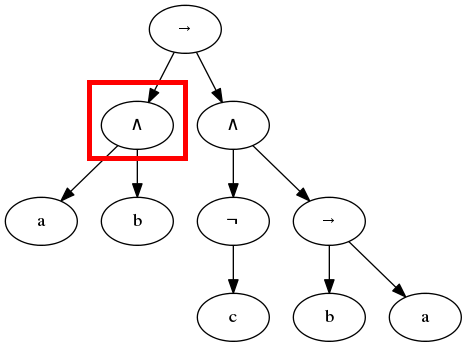
\includegraphics[scale=0.45]{t6.png}
\end{figure}

\FloatBarrier

могут быть следующие формулы:

\FloatBarrier

\begin{figure}[!h]
  \centering
    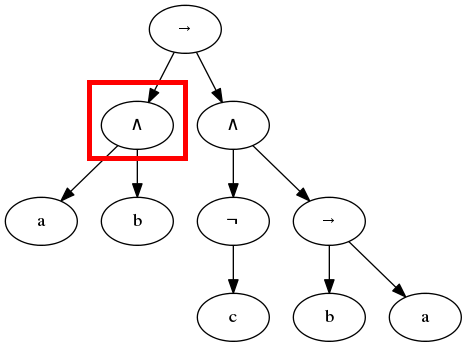
\includegraphics[scale=0.45]{t7.png}
\end{figure}

\begin{figure}[!h]
  \centering
    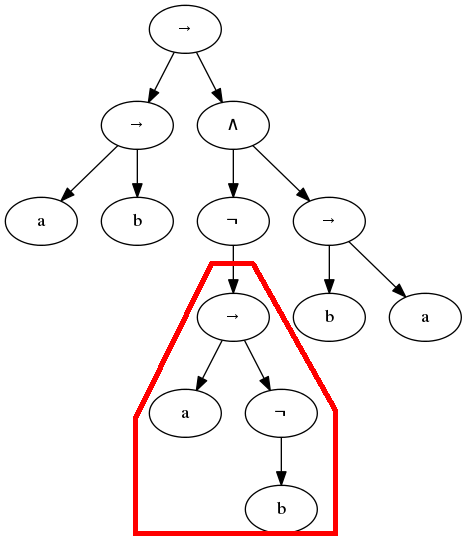
\includegraphics[scale=0.45]{t8.png}
\end{figure}

\begin{figure}[!h]
  \centering
    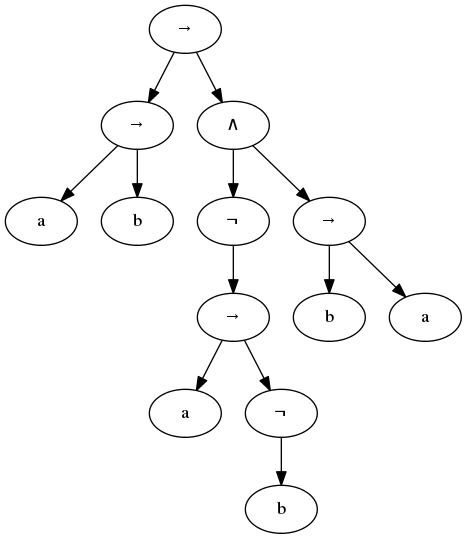
\includegraphics[scale=0.45]{t9.png}
\end{figure}

\begin{figure}[!h]
  \centering
    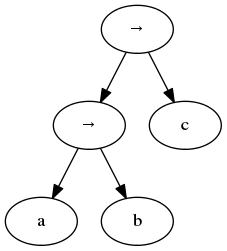
\includegraphics[scale=0.45]{t10.png}
\end{figure}

\FloatBarrier

\subsection{Многокритериальная оптимизация}

Многокритериальная оптимизация --- это процесс одновременной оптимизации двух или более конфликтующих целевых функций
в заданной области определения. В качестве критерия оптимальности будем использовать оптимальность по Парето:
говорят, что одно решение доминирует над другим, если оно по всем критериям не хуже другого и как минимум по одному
строго лучше. Множеством оптимальных решений называются решения, над которыми никто не доминирует. Таким образом
в качестве результата работы алгоритма будет получен фронт решений, являющихся оптимальными.

\begin{figure}[!hb]
  \centering
    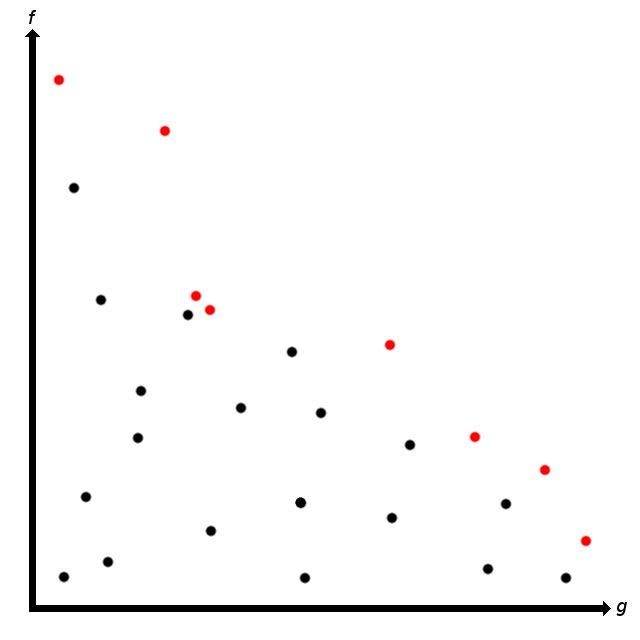
\includegraphics[scale=0.4]{opt.png}
  \caption{Красным цветом отмечены оптимальные решения задачи оптимизации функций $f$ и $g$.}
\end{figure}

\subsection{Постановка задачи}

Пусть задан входной автомат $a$. Требуется найти удовлетворяющие ему формулы, оптимальные в смысле ранее указанных
двух свойств. Формализуем их.

Пусть $A_f$ --- множество всех возможных автоматов, удовлетворяющих некоторой формуле $f$. Будем считать,
что чем меньше мощность $A_f$, тем больше информации о входном автомате $a$ несет формула.

Пусть есть множество операторов $O$ и множество пропозициональных переменных $V$.
Тогда каждому оператору $o \in O$ и утверждению $v \in V$ сопоставим их веса $w_o$ и $w_v$, соответственно.
Введем понятие веса формулы таким образом:
\begin{equation*}
\text{weight}(v) = w_v, \text{weight}(o(arg_1\; \ldots \; arg_n)) = w_o + \sum_{i=1}^{n}\text{weight}(arg_i).
\end{equation*}
Будем искать формулы минимального веса, формализовав таким образом требование простоты формулы.

\section{2. Предлагаемый алгоритм}

Для решения задачи будем использовать генетическое программирование \cite{kz1}. Будем представлять формулу в виде дерева разбора.
Для генерации, скрещивания и мутации формул будем использовать стандартные алгоритмы генетического программирования,
реализованные в библиотеке эволюционных алгоритмов ECJ (http://cs.gmu.edu/~eclab/projects/ecj) и описанные в \cite{kz1, kz2}.
Так как в качестве целевых были выделены сразу несколько критериев, то будем использовать многокритериальную оптимизацию.

В качестве конкретных реализаций многокритериальной оптимизации были испробованы алгоритмы NSGA-II \cite{nsga2} и SPEA2 \cite{spea2}.
При одинаковых результатах SPEA2 работал существенно быстрее и был выбран для дальнейшего использования. Алгоритм SPEA2,
наряду с популяцией, использует архив. Начав с пустым архивом $A_0$ и сгенерированной популяцией $P_0$, алгоритм до
тех пор, пока не выполнено одно из завершающих условий, выполняет следующие шаги: 

1. Назначить каждой особи $i$ из $P_t$ и $A_t$ значение функции приспособленности
$$
F(i) = \frac{1}{d_k(i) + 2} + \sum_{j\in P_t + A_t, j > i}|\{k|k \in P_t + A_t \wedge k > j\}|
$$
Где $d_k$ --- расстояние до k-ой ближайшей особи (обычно берут $k = \sqrt{|P| + |A|}$), > --- отношение доминирования по Парето.

2. Скопировать оптимальные особи из $P_t$ и $A_t$ в $P_{t+1}$ (при необходимости архив обрезается или дополняется неоптимальными решениями).

3. С помощью бинарного турнира выбрать особи из $A_{t+1}$ для скрещивания с целью получения новой популяции. 

В качестве критериев оптимизации будем использовать: удовлетворение входного автомата формуле, минимальность веса
формулы и минимальность числа автоматов, которым удовлетворяет формула. Очевидно, однако, что вычисление последнего
критерия не представляется возможным даже при условии небольшого числа состояний в автомате. Поэтому в дальнейшем будут
рассмотрены несколько критериев и их комбинаций, эффективно приближающих требуемое. Позже будет приведен
анализ качества их работы.

В данной работе ограничимся генерацией формул вида $G(\ldots)$, то есть таких, которые выполняются в любой момент времени.
Система типов ECJ позволяет сопоставить каждому узлу дерева особи его тип. Тип узла
определяет количество и типы его поддеревьев. ECJ будет генерировать только корректно типизирующиеся особи.
Таким образом мы можем накладывать на них определенные ограничения. В частности мы запретим генерацию следующих
комбинаций: $\lnot(\lnot(\ldots))$, $F(F(\ldots))$, $F(X(\ldots))$, $X(F(\ldots))$, $G(X(\ldots))$, так как
они имеют более простые аналоги, по смыслу ничем или слабо отличающиеся от указанных.

\subsection{Критерий 1. Входной автомат должен удовлетворять формуле.}

Будем определять удовлетворяет ли автомат $a$ формуле $f$ с помощью верификатора автоматных программ, разработанного в \cite{eg}.
Верификатор возвращает число $r(a, f) = \frac{\text{verifiedTransitions}(a, f)}{\text{totalTransitions}(a)}$ --- отношение числа
переходов, которым формула удовлетворяет, к общему числу переходов. Таким образом, значения $r(a, f)$ лежат в отрезке $[0, 1]$; и равно
единице, тогда и только тогда, когда автомат удовлетворяет формуле.

\subsection{Критерий 2. Минимальность веса формулы.}

Ранее для каждой формулы $f$ был введен ее вес $\text{weight}(f)$. Используем в качестве критерия число $c_2 = \frac{1}{\text{weight}(f)}$.
В качестве весов операторов и утверждений выберем числа, большие или равные единице.
В таком случае $c_2 \in [0, 1]$ и максимально при минимальном весе формулы.

\subsection{Критерий 3. Число случайных автоматов, удовлетворяющих формуле.}

Сгенерируем некоторое число $N$ случайных автоматов с теми же множествами состояний, входных и выходных событий, что и
у исходного. Для каждого из полученных автоматов измерим с помощью верификатора, насколько он удовлетворяет формуле.
Получим $N$ чисел $r_i$ из промежутка $[0, 1]$. В качестве результата возьмем величину $c_3 = \frac{1}{1 + \sum_{i = 1}^{N}r_i^2}$.

\subsection{Критерий 4. Число мутантов исходного автомата, удовлетворяющих формуле.}

Возьмем исходный автомат и сгенерируем для него некоторое число мутантов --- исходных автоматов с небольшими
случайными изменениями функций переходов $\phi$ и выходов $\delta$. Будем использовать следующие операторы мутации.

1. \textbf{Изменение состояния, в которое ведет переход.} Для случайно выбранного перехода в автомате состояние $y$,
в которое он ведет, заменяется на другое состояние, случайно выбранное из $Y \textbackslash \{y\}$. 

2. \textbf{Добавление или удаление переходов.} Для каждого состояния с определенной вероятностью изменим набор переходов.
Случайным образом решается добавить или удалить переход. В случае добавления перехода добавим новый переход из
текущего состояния в некоторое случайно выбранное состояние. В случае удаления из текущего состояния удаляется
случайно выбранный переход.

В качестве результата используем величину, аналогичную результату для случайных автоматов.

\subsection{Критерий 5. Удовлетворение автомата, построенного по сценариям, формуле.}

Сценарий --- некоторый случайный путь фиксированной длины в автомате. Построим для входного автомата некоторое
число сценариев. На основе этих сценариев построим новый автомат $a^*$ при помощи алгоритма, описанного в \cite{eg}.
Заметим, что полученный автомат может удовлетворять не всем формулам, верным для исходного автомата, так как
длина любого сценария конечна. В качестве результата используем величину $c_5 = 1 - r(a^*, f)$.

\subsection{Критерий 6. Число мутантов автомата, построенного по сценариям, удовлетворяющих формуле.}

Критерий аналогичен критерию номер четыре с тем лишь отличием, что мутанты строятся на основе автомата, построенного по
сценариям, а не исходного.

\section{3. Результаты}

\subsection{Проведенные испытания}

Для тестирования алгоритма использовался автомат, управляющий дверьми лифта, описанный в \cite[Sec 2.3.1]{eg}.

\begin{figure}[!hb]
  \centering
    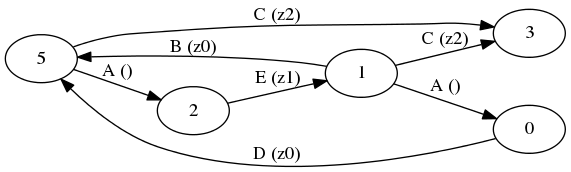
\includegraphics[scale=0.5]{lift.png}
  \caption{Автомат, управляющий дверьми лифта}
\end{figure}

Состояние под номером ноль --- начальное. Автомат принимает следующие события:

$\bullet$ $A$ --- двери лифта полностью открылись или закрылись;

$\bullet$ $B$ --- закрытию дверей мешает препятствие;

$\bullet$ $C$ --- поломка дверей лифта;

$\bullet$ $D$ --- нажата кнопка ``Открыть двери'';

$\bullet$ $E$ --- нажата кнопка ``Закрыть двери''.

Автомат имеет три выходных воздействия:

$\bullet$ $z_0$ --- приступить к открытию дверей;

$\bullet$ $z_1$ --- приступить к закрытию дверей;

$\bullet$ $z_2$ --- сообщить в аварийную службу о поломке лифта.

Автомат был построен на основе следующей спецификации:
\begin{multline*}
G(\text{wasEvent}(D) \rightarrow \text{wasAction}(z_0))\\
G(\text{wasEvent}(E) \leftrightarrow \text{wasAction}(z_1))\\
G(\text{wasEvent}(C) \leftrightarrow \text{wasAction}(z_2))\\
G(\text{wasEvent}(B) \rightarrow \text{wasAction}(z_0))\\
G(\text{wasEvent}(A) \rightarrow X(\text{wasEvent}(D) \vee \text{wasEvent}(E)))\\
G(\text{wasEvent}(D) \rightarrow X(\text{wasEvent}(A) \vee \text{wasEvent}(C)))\\
G(\text{wasAction}(z_0) \rightarrow X(\text{wasEvent}(A) \vee \text{wasEvent}(C)))\\
G(\text{wasEvent}(E) \rightarrow X(\text{wasEvent}(A) \vee \text{wasEvent}(B) \vee \text{wasEvent}(C)))\\
G(\text{wasAction}(z_0) \rightarrow X(U(\lnot \text{wasAction}(z_0), \text{wasAction}(z_1) \vee \text{wasEvent}(C))))\\
G(\text{wasAction}(z_1) \rightarrow X(U(\lnot \text{wasAction}(z_1), \text{wasAction}(z_0) \vee \text{wasEvent}(C))))\\
\lnot F(\text{wasEvent}(C) \wedge X(F(\text{wasEvent}(D) \vee \text{wasEvent}(E) \vee \\ \vee \text{wasEvent}(A) \vee \text{wasEvent}(B) \vee \text{wasEvent}(C))))
\end{multline*}

Проведено несколько запусков различных конфигураций алгоритма. Во всех конфигурациях использовались первые два критерия.
Для оставшихся четырех критериев были испытаны все комбинации. Всего таким образом было получено шестнадцать конфигураций.
Число поколений в каждом испытании --- 50, размер популяции --- 500, размер архива --- 100.

\begin{table}
\centering
\caption{Конфигурации}
\begin{tabular}{ l | l | l | l | l | l | l }
конфигурация \textbackslash \ критерий & 1 & 2 & 3 & 4 & 5 & 6 \\
\hline
1  & + & + & - & - & - & - \\
2  & + & + & - & - & - & + \\
3  & + & + & - & - & + & - \\
4  & + & + & - & - & + & + \\
5  & + & + & - & + & - & - \\
6  & + & + & - & + & - & + \\
7  & + & + & - & + & + & - \\
8  & + & + & - & + & + & + \\
9  & + & + & + & - & - & - \\
10 & + & + & + & - & - & + \\
11 & + & + & + & - & + & - \\
12 & + & + & + & - & + & + \\
13 & + & + & + & + & - & - \\
14 & + & + & + & + & - & + \\
15 & + & + & + & + & + & - \\
16 & + & + & + & + & + & + \\
\end{tabular}
\end{table}

Для оценки результатов будем, во-первых, анализировать полученные формулы вручную. Формулы, сообщающие некоторые тривиальные
факты, например: ``В любой момент времени либо что-то мешает закрытию дверей либо нет'', нас не интересуют.
Так же не подходят чрезмерно сложные и громоздкие формулы. Примером хороших формул может служить приведенная ранее спецификация.

Во-вторых, наряду с анализом полученных формул вручную будем использовать следующую величину.
Построим на основе выведенных формул и сценариев автомат. Возьмем набор формул, написанных человеком для исходного автомата, и
проверим, скольким из них удовлетворяет построенный автомат. Чем больше эта величина, тем больше информации об исходном
автомате нам дают выведенные формулы.

\subsection{Результаты испытаний}

Было проведено десять запусков каждой из шестнадцати конфигураций. Суммарное время работы составило чуть менее семнадцати часов.
Спецификация, содержащая семнадцать формул была взята из \cite{eg}.
Таким образом то, насколько много информации дают формулы, полученные с помощью некоторой конфигурации, о входном автомате,
характеризуется числом от 0 до 170.

Максимальный результат --- 170 набрала реализация номер шестнадцать. Второе место с результатом 169 разделили две реализации:
номер десять и номер четырнадцать. Третье место (164) так же заняли две реализации: номера семь и двенадцать.
Далее приведены примеры сгенерированных формул. 

\begin{multline*}
G(F(\text{wasAction}(z_1)) \rightarrow \lnot \text{wasAction}(z_2))\\
G(X(\text{wasAction}(z_1)) \rightarrow \text{wasEvent}(A))\\
G(\text{wasAction}(z_0) \rightarrow F(\text{wasAction}(z_1) \vee X(\text{wasAction}(z_2))))\\
G(X(\text{wasEvent}(A)) \rightarrow (\text{wasAction}(z_1) \vee \text{wasAction}(z_0)))\\
\end{multline*}

\section{4. Заключение}

Разработан метод генерации LTL-формул по управляющему конечному автомату и написана программа на языке программирования Java
(https://github.com/V1489Cygni/ltlgen), являющаяся модулем для библиотеки ECJ и реализующая этот метод.
Были протестированы различные конфигурации алгоритма и выбраны лучшие из них. При тестировании алгоритм показал
достаточно стабильные результаты, было получено достаточное количество формул, удовлетворяющих поставленной цели.

\begin{thebibliography}{10}

\bibitem{tl}A. Pnueli. The temporal logic of programs. In Foundations of Computer Science, 1977., 18th Annual Symposium on, pages 46–57, Oct 1977.

\bibitem{sm1}V. Dallmeier, C. Lindig, A. Wasylkowski, and A. Zeller. Mining object behavior with adabu. In Proceedings of the
2006 International Workshop on Dynamic Systems Analysis, WODA ’06, pages 17–24, New York, NY, USA, 2006. ACM.

\bibitem{sm2}M. D. Ernst, J. Cockrell, W. G. Griswold, and D. Notkin. Dynamically discovering likely program invariants to support program evolution. In
Proceedings of the 21st International Conference on Software Engineering, ICSE ’99.

\bibitem{sm3}M. Gabel and Z. Su. Javert: Fully automatic mining of general temporal properties from dynamic traces. In Proceedings of the 
16th ACM SIGSOFT International Symposium on Foundations of Software Engineering, SIGSOFT ’08/FSE-16, pages 339–349, New York, NY, USA, 2008. ACM.

\bibitem{sm4}J. Yang, D. Evans, D. Bhardwaj, T. Bhat, and M. Das. Perracotta: Mining temporal api rules from imperfect traces. In Proceedings of the 28th
International Conference on Software Engineering, ICSE ’06, pages 282–291, New York, NY, USA, 2006. ACM.

\bibitem{kz1}John R. Koza. Genetic Programming: On the Programming of Computers by Means of Natural Selection. MIT press, 1992.

\bibitem{kz2}John R. Koza. Genetic Programming II: Automatic Discovery of Reusable Programs. MIT press, 1994.

\bibitem{nsga2}Kalyanmoy Deb, Amrit Pratap, Sameer Agarwal, T. Meyarivan. A Fast and Elitist Multiobjective Genetic Algorithm: NSGA-II.

\bibitem{spea2}Eckart Zitzler, Marco Laumanns, Lothar Thiele. SPEA2: Improving the Strength Pareto Evolutionary Algorithm. //
Computer Engineering and Networks Laboratory (TIK)
Department of Electrical Engineering
Swiss Federal Institute of Technology (ETH) Zurich
ETH Zentrum, Gloriastrasse 35, CH-8092 Zurich, Switzerland.

\bibitem{eg}Егоров Кирилл Викторович. Генерация управляющих автоматов на основе генетического программирования и верификации: 
Диссертация на соискание ученой степени кандидата технических наук. 2013.   

\end{thebibliography}

\end{document}
